\documentclass[11pt,a4paper]{ctexart}
\usepackage[a4paper,margin=1.55cm]{geometry}
\usepackage{array}
\usepackage{tabularx}
\usepackage{enumitem}
\usepackage{graphicx}
\usepackage{xcolor}
\usepackage{hyperref}
\usepackage{setspace}
\usepackage{titlesec}
\usepackage{fancyhdr}
\usepackage{tikz}

\definecolor{Accent}{HTML}{1F2937}
\definecolor{TextGray}{HTML}{374151}
\definecolor{LightGray}{HTML}{6B7280}

\hypersetup{colorlinks=true,urlcolor=Accent,linkcolor=Accent}
\pagestyle{fancy}
\fancyhf{}
\renewcommand{\headrulewidth}{0pt}
\renewcommand{\footrulewidth}{0pt}
\cfoot{\textcolor{LightGray}{詹绍基 | 简历}}

\titleformat{\section}{\large\bfseries\color{Accent}}{}{0em}{}
\titlespacing*{\section}{0pt}{9pt}{5pt}
\setlist[itemize]{leftmargin=1.6em,itemsep=2pt,topsep=2pt}
\setlength{\parindent}{0pt}
\linespread{1.14}

\begin{document}

\noindent
\begin{minipage}[t]{0.76\textwidth}
{\LARGE\bfseries\color{Accent} 詹绍基}

\vspace{5pt}
\textcolor{TextGray}{手机：18550954831 \quad 邮箱：\href{mailto:z1309457869@163.com}{z1309457869@163.com}}

\vspace{3pt}
\textcolor{TextGray}{出生：2000.10 \quad 城市：珠海}

\vspace{4pt}
\textcolor{TextGray}{研究关键词：脉冲神经网络（SNN）、神经可塑性、具身智能、隐私与能效协同优化、可信评测}
\end{minipage}
\hfill
\begin{minipage}[t]{0.2\textwidth}
\raggedleft
\setlength{\fboxsep}{1.5pt}
\color{LightGray}\fbox{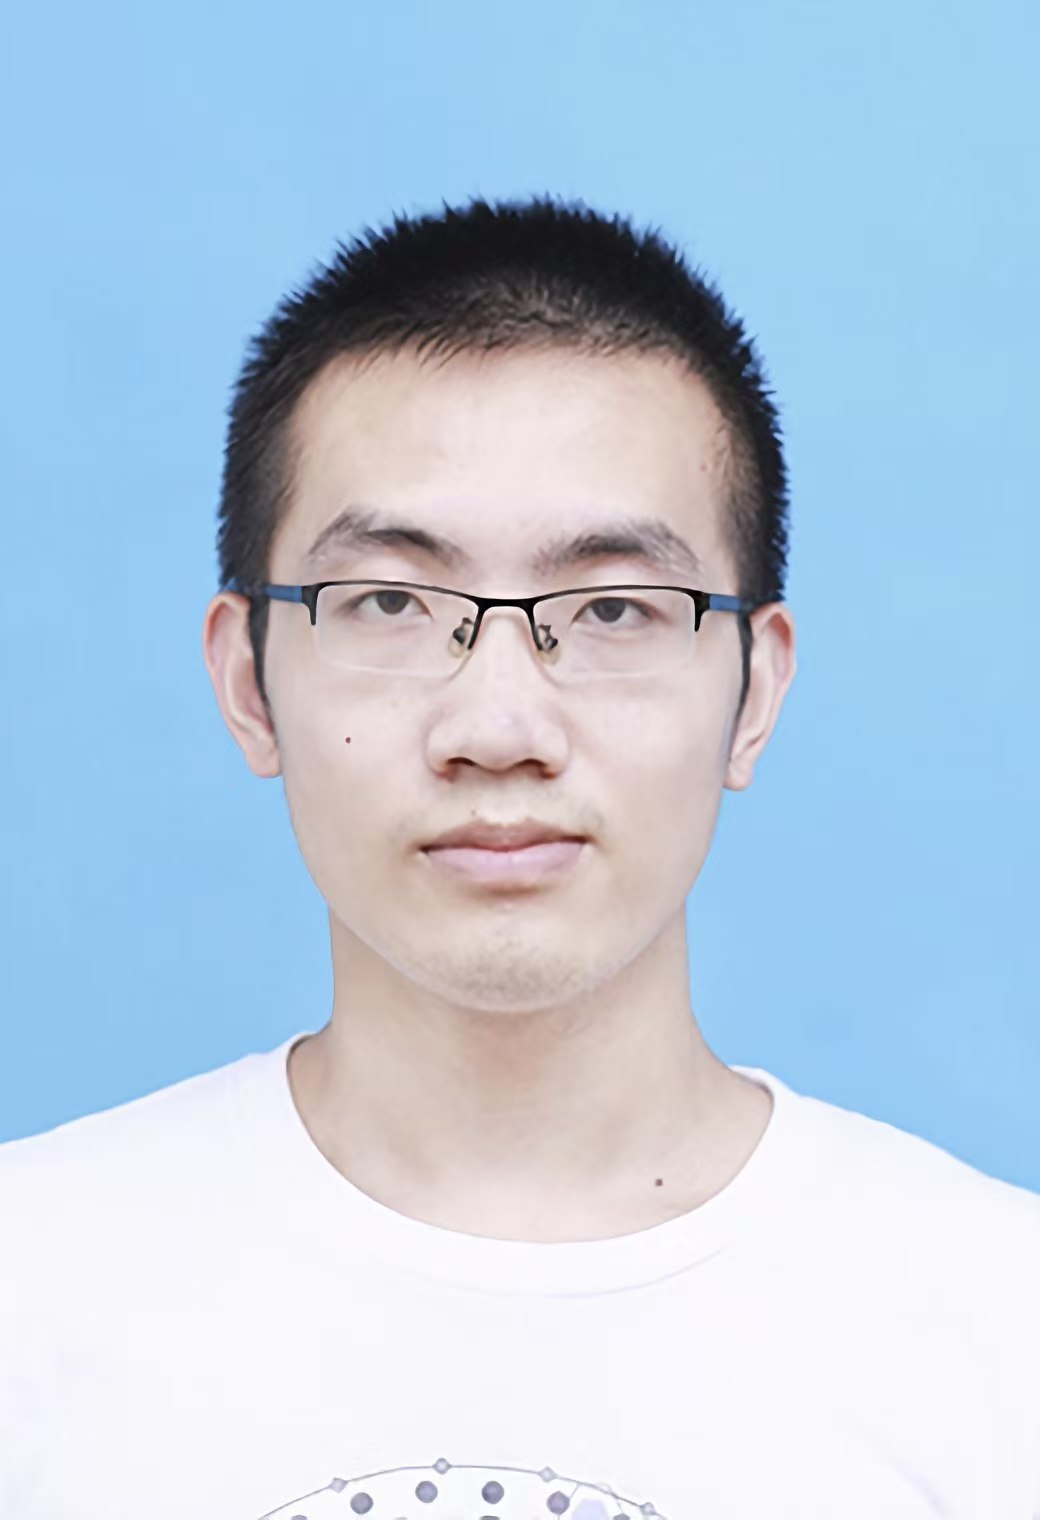
\includegraphics[width=2.55cm,height=3.35cm,keepaspectratio]{resume_photo.jpg}}
\end{minipage}

\vspace{4pt}
\noindent\textcolor{LightGray}{\rule{\textwidth}{0.5pt}}

\section*{教育背景}
\begin{tabularx}{\textwidth}{>{\bfseries}p{2.2cm}Xr}
本科 & 苏州大学，医学影像学（辅修计算机） & 2019.09--2024.06 \\
二学士 & 北京师范大学，法学（第二学士学位） & 2024.09--2026.07（预计） \\
考试成绩 & 2026考研初试总分329（英语一、数学一、843互联网创新设计），CET-6：595 & \\
\end{tabularx}

\section*{科研与工程能力}
\begin{itemize}
  \item \textbf{SNN建模与训练：} LIF神经元建模、代理梯度训练、时间步展开训练、STDP与奖励调制可塑性实现与比较。
  \item \textbf{可信AI评测：} 成员推断攻击（MIA）、DP-SGD参数扫描、隐私-性能-能效三目标协同分析。
  \item \textbf{实验工程化：} 基于PyTorch构建可复现实验流水线，支持多seed统计、置信区间汇总、自动图表与报告生成。
  \item \textbf{数据与任务：} 医疗影像（PathMNIST、DermaMNIST）、脑机接口解码（BCI流程搭建）、合成数据快速验证。
  \item \textbf{研究执行：} 可独立完成问题定义、实验设计、结果解释、文档沉淀与复现实验打包，可按不同课题方向快速适配任务。
\end{itemize}

\section*{重点项目经历（独立开发）}
\textbf{1. EmbodiedSNNPrototype：具身闭环脉冲神经网络原型}
\begin{itemize}
  \item 搭建 environment $\rightarrow$ sensory encoding $\rightarrow$ LIF brain $\rightarrow$ motor readout $\rightarrow$ environment 的具身闭环系统，重点研究网络连接结构与行为输出的关系。
  \item 设计并实现 structured / structured\_plastic / structured\_rewired / random\_sparse 多连接模式，支持噪声、重连率、饥饿驱动、可塑性学习率与衰减等参数扫描。
  \item 构建统一目标函数并完成批量benchmark排序，最优structured\_plastic配置在综合目标上领先（objective\_mean=2.0327）。
  \item 关键行为指标：food\_eaten\_mean=3.24，near\_food\_ratio\_mean=0.5367，验证“结构先验 + 局部可塑性”在闭环任务中的有效性。
  \item 输出内容：可复现实验配置、结果表与分析报告，为后续“可塑性规则自动搜索”课题奠定基础。
\end{itemize}

\textbf{2. Neuro-Symbiosis：SNN-Transformer脑机解码与三目标协同优化}
\begin{itemize}
  \item 构建SNN前端 + Transformer时序解码后端的混合架构，面向BCI任务联合优化效用（accuracy/F1）、隐私（MIA/AUC）与能效（latency/energy）。
  \item 打通完整实验链：预处理、训练、baseline对比、隐私评估、能耗评估、DP-SGD sweep、多seed鲁棒性统计与汇总报告。
  \item 设计SNN/Transformer/Hybrid三类基线与统一评估协议，支持Pareto视角比较不同模型在三目标上的权衡关系。
  \item 形成可证伪研究问题：spike rate与有效token长度如何共同影响总能耗及隐私-性能权衡，为后续机制研究提供量化抓手。
  \item 工程状态：LOSO流程与脚本接口已搭建，具备在真实受试者级数据上快速扩展的条件。
\end{itemize}

\textbf{3. MedSparseSNN：医疗影像中的稀疏SNN隐私-效率研究}
\begin{itemize}
  \item 在DermaMNIST与PathMNIST系统对比SNN / DenseSNN / ANN的准确率、成员推断风险、延迟与能效指标。
  \item PathMNIST结果：SNN test\_acc=82.33$\pm$0.31（ANN为85.12$\pm$0.40）。
  \item 在PathMNIST上，SNN理论有效MAC节省84.18\%$\pm$0.52\%，在性能接近前提下体现显著稀疏计算优势。
  \item DermaMNIST结果：SNN test\_acc=69.93$\pm$0.20，理论有效MAC节省90.74\%$\pm$0.23\%，验证稀疏发放在跨数据集场景中的可迁移性。
  \item 隐私侧完成黑盒MIA评估（accuracy/AUC/F1/precision/recall），形成“隐私结论需结合数据域解释”的审慎分析框架。
  \item 沉淀产物包含训练脚本、攻击脚本、实验报告与图表素材，可直接支撑复试答辩与进一步论文化工作。
\end{itemize}

\textbf{4. PrivEnergyBench：隐私-能效-效用三目标评测工具箱}
\begin{itemize}
  \item 将训练、MIA、时延、能耗代理整合为统一benchmark工具链，支持linear/MLP/CNN1D/Transformer四类基线模型。
  \item 支持多seed自动汇总mean/std/95\%CI，并自动输出CSV、Markdown报告、Pareto图与HTML dashboard。
  \item 默认3-seed结果：MLP最高val\_acc=0.9208；Linear最低能耗0.0164 mJ/sample，形成可复用的三目标权衡展示案例。
  \item 项目价值在于将一次性实验脚本沉淀为稳定评测基础设施，提升跨项目比较的一致性与复现效率。
\end{itemize}

\section*{研究关注与下一步计划}
\begin{itemize}
  \item \textbf{研究主线：} 在资源受限与隐私约束下，探索SNN及混合模型在效用、鲁棒性与能效之间的最优平衡。
  \item \textbf{近期计划（6-12个月）：} 深化可塑性规则搜索、推进真实BCI受试者级评测、完善隐私攻击与防御对照实验。
  \item \textbf{中期目标：} 形成可复现实验基准与高质量研究文档，逐步收敛为可投稿的问题定义与实验结论。
\end{itemize}

\section*{补充经历与证明}
\begin{itemize}
  \item 上海交通大学医学院苏州九龙医院临床实习（2023.06--2024.06）：完成多科室轮转，出科考试平均93分，完成影像报告300+份，综合合格率96\%。
  \item 证明材料可提供：本科毕业证/学位证/成绩单、学信网学籍学历验证报告、学位在线验证报告、考研初试成绩证明。
  \item 开源主页：\href{https://github.com/ZhanMous}{https://github.com/ZhanMous}
\end{itemize}

\end{document}
